\documentclass[11pt,a4paper,titlepage,openright]{report}
\usepackage[utf8]{inputenc}
\usepackage[T1]{fontenc}
\usepackage[french]{babel}
\usepackage[top=1.5cm, bottom=5cm]{geometry}
\usepackage{fancyhdr, graphicx, array, hyperref}
\usepackage{glossaries}

\pagestyle{fancy}

\title{\textsc{\textbf{Gestion de la configuration\\Interpréteur du langage LIR}}}
\date{}
\author{Nicolas \textsc{Caminade} \and Sylvan \textsc{Courtiol} \and Pierre \textsc{Debas} \and Heïa \textsc{Dexter} \and Lucàs \textsc{Vabre} }
\begin{document}
    \lhead{Gestion de la configuration}
    \rhead{
        
\includegraphics[width=2cm]{img/logoiut}
    }

    \cfoot{\thepage}
    \headheight = 2cm
    \headsep = 1.5cm


    \begin{titlepage}
        \fontfamily{pag}\selectfont

        \begin{center}\normalsize
            \MakeUppercase{IUT de Rodez \hfill Département informatique \hfill INFO1 2020-2021}
        \end{center}
        \vspace*{0.1cm}
        \hrule
        \vspace*{0.2cm}
        \begin{flushright}
            
\includegraphics[width=4cm]{img/logoiut}
        \end{flushright}
        \vspace*{2cm}
        \begin{flushright}\Huge
            \textsc{\textbf{Gestion de la configuration\\Interpréteur du langage LIR}}
        \end{flushright}
        \hrule
        \begin{flushleft}
            \MakeUppercase{Projet proposé par Frédérique Barrios}
        \end{flushleft}
        \vspace*{1cm}
        \begin{center}\normalsize
        	\textbf{version : \today}
        \end{center}
        \vspace*{1cm}
        \begin{center}\Large
            Nicolas \textsc{Caminade}, Sylvan \textsc{Courtiol},\\
            Pierre \textsc{Debas}, Heïa \textsc{Dexter}, \\
            Lucàs \textsc{Vabre}
        \end{center}
        \vfill
        \begin{center}\normalsize
            \MakeUppercase{Projet tuteuré --- Semestre 2}
        \end{center}
    \end{titlepage}


    % Sommaire
    \renewcommand{\contentsname}{Sommaire}
    \tableofcontents
    
    \newpage

    % numérotation des sections et sous-section indiféremment des chapitres
    \setcounter{section}{0}
    \renewcommand{\thesection}{\arabic{section}} 
    \renewcommand{\thesubsection}{\arabic{section}.\arabic{subsection}}
    
    
    \section*{Introduction}
    \Large
    Ce document a pour but de confirmer par écrit la configuration logicielle choisie pour le
    projet.
    \par Le contenu de ce document n’est pas fixé et des changements peuvent être apportés. Cependant ce document doit être connu et suivi par les membres du groupe. En cas de modifications, une annonce sur discord sera faite.
    \par Pour toute question ou suggestion se référer au gestionnaire de configuration (présentement
    Sylvan COURTIOL).


    \normalsize
    \section{Logiciels de développement}
        \subsection{Environnement de Développement Intégré}
        Eclipse JEE (version 2020-12)
        \par JDK 15
        \par Les tests unitaires seront fait avec l'outil créé en TD de Programmation Orienté Objet par M. Barrios.
        
        \subsection{Contrôle des versions du code}
        Git avec dépôt sur GitHub. Utilisation de GitHub Desktop pour l'utlisation de git avec une interface graphique.
        
        \subsection{Organisation}
        Via le site Trello.
        
        \subsection{Modélisation}
        La modélisation UML sera effectuée sur Modelio Open Source (version 4.1).
        
    \section{Logiciels généraux}
        \subsection{Communication}
        \par Les communications formelles écrites sont effectuées via les mails de l’IUT (généralement par le chef
        de projet) avec les autres membres du projet en CC.
        \par Les réunions entre la MOA et la MOE se feront de préférence en présentiel avec si possible tous les membres du groupe présents. Cependant au vu de la situation sanitaire et des restrictions en vigueurs certains membres peuvent être dans l'impossibilité de venir en présentiel. Dans ce cas les membres concernés assisteront à la réunion par visioconférence via Google Meet.
        \par Serveur discord spécifique au projet pour la communication écrite ou vocale interne à la MOE.
        
        
        \subsection{Éditeur de texte}
        Le traitement de texte sera fait sous LaTex notamment avec la distribution MiKTex et l'IDE TexStudio. Les documents texte sont partagés en PDF ou version papier à la MOA/MOE  et en format modifiable .tex seulement à la MOE via la solution de partage distant des fichiers (voir sous-section suivante).
        
        \subsection{Partage distant des fichiers}
        Les partages de tous les fichiers généraux et codes sources se feront sur GitHub via le site, le logiciel GitHub desktop ou git. Les échanges des fichiers généraux se feront plus précisément dans la branche main. Il y aura également une intégration Discord informant des commits.
        
    \section{Sécurité}
    \par Si possible tous les membres du groupe auront les mêmes droits sur les fichiers communs.
    En conséquence aucun membre du groupe ne doit donner des droits sur ces fichiers à une
    personne extérieure au projet (autre que MOA).
    \par Les sauvegardes du dépôt GitHub (contenant toutes les données du projets) seront effectuées
    régulièrement (tous les 1 ou 2 jours) par le gestionnaire de configuration. Toutes données qui ne
    sont pas dans le dépôt sont à la responsabilité de chacun.
    Les sauvegardes sont enregistrée en local par le gestionnaire de configuration ainsi que sur le Google drive partagé du projet.



    \appendix
    %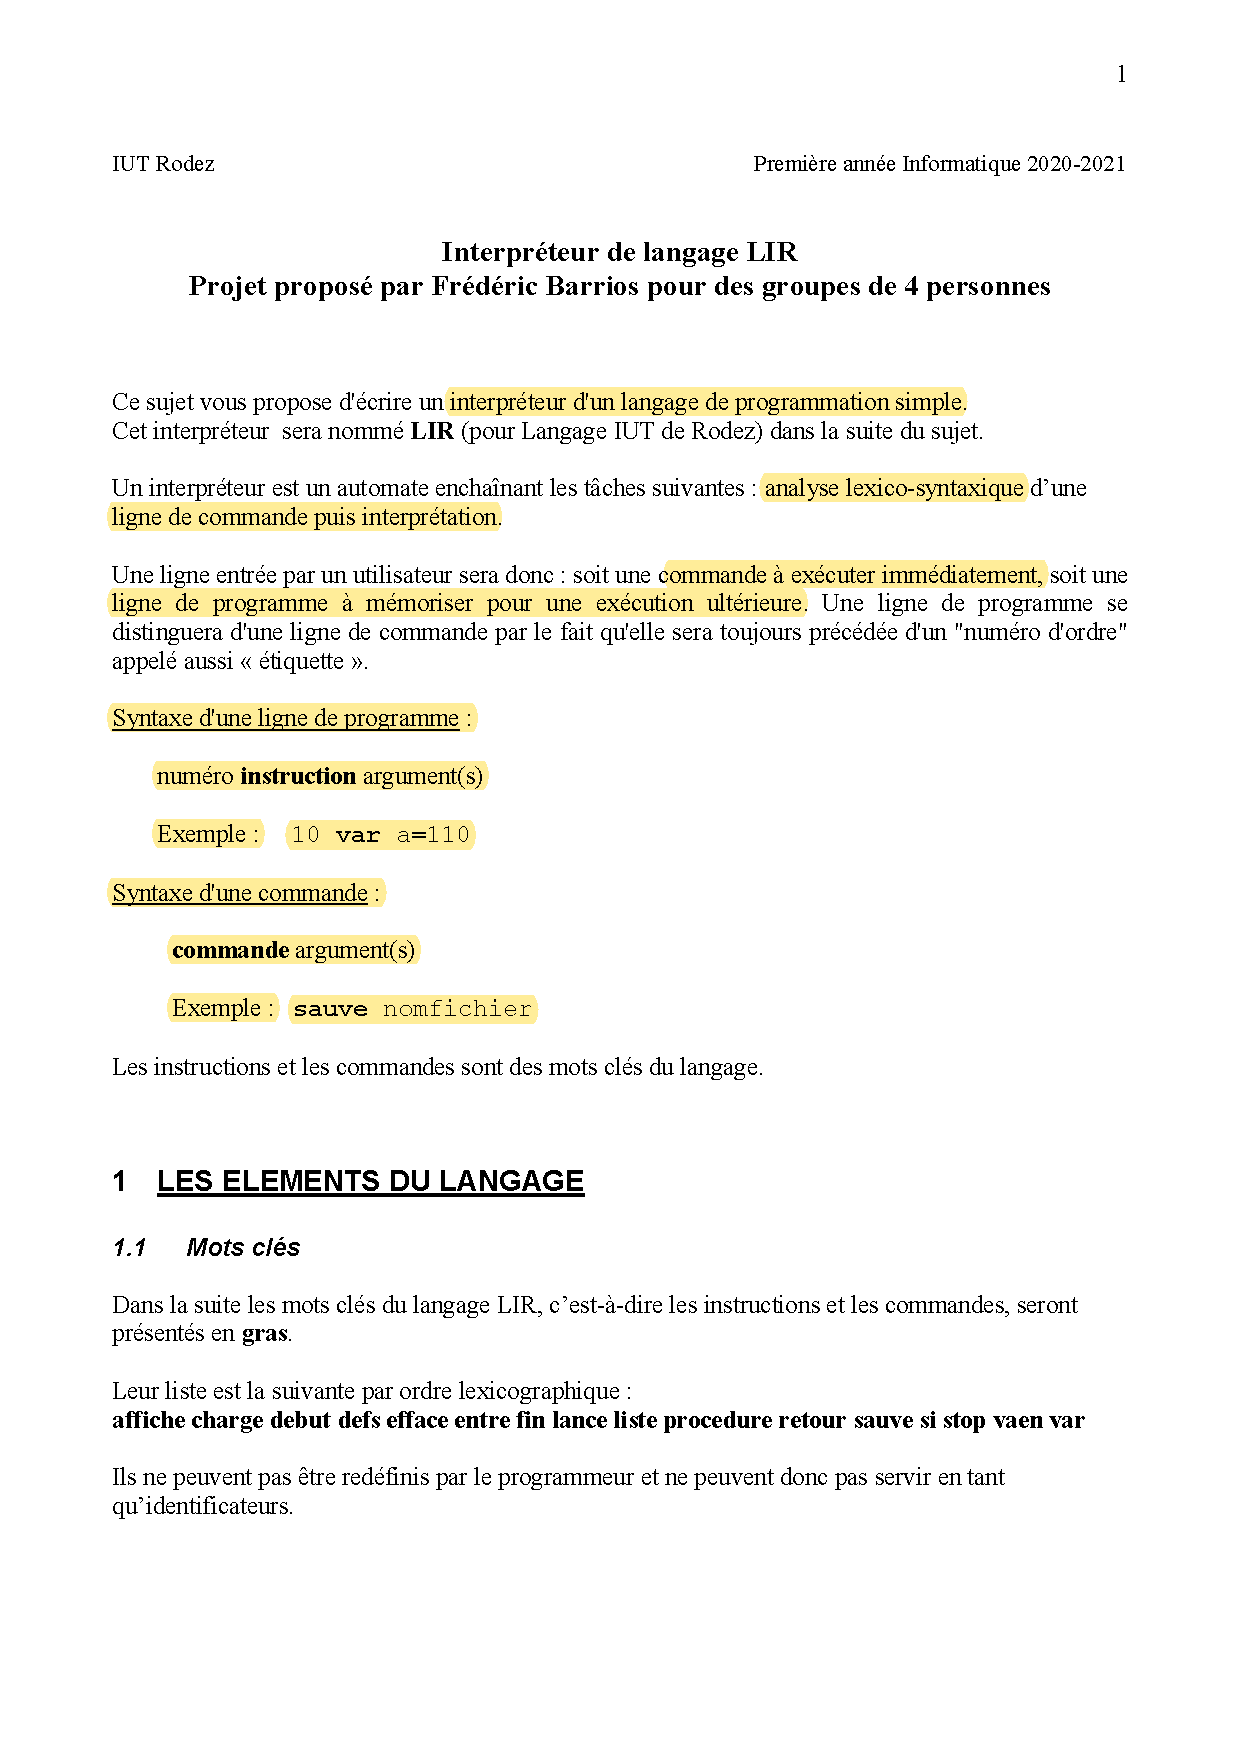
\includepdf[pages=-]{fichiers/BarriosInterpreteurLIR2021}

\end{document}